% ==========================================
% SECTION 2: TECHNICAL DEVELOPMENT (40%)
% ==========================================
\section{Technical Development}

\subsection{Source Materials (5\%)}
The conceptualisation and development of the Competitor Benchmarking System were grounded in three primary categories of source materials:

\begin{itemize}
    \item \textbf{Stakeholder Requirements \& Domain Knowledge:} The primary source was the consultation with the Strategic Planning and Insight Office (SPIO). Key artifacts included the client's existing manual Excel workflows and the "S-Squared" commercial dataset. These established the baseline for the data schema (specifically the distinction between 'Home' and 'International' fees and 'Course Options') and defined the "Must-Have" features for the MVP.
    \item \textbf{Target Web Specifications (DOM Analysis):} To develop the scraping engine, we analysed the document object models (DOM) of the 35 target university websites. This analysis revealed a "Dual Certainty Profile": some sites yielded data via static HTML (suitable for lightweight parsing via Cheerio), while others (e.g., University of Edinburgh) relied on Single Page Application (SPA) frameworks, necessitating a headless browser approach (Puppeteer).
    \item \textbf{API Documentation:} The UCAS Open Data API served as the authoritative source for course titles and entry requirements. This documentation allowed us to design a "Hybrid Ingestion Pipeline," reducing the load on custom web scrapers by only scraping data (like specific fees) that is not available via UCAS.
\end{itemize}

\subsection{Technical Description (30\%)}

\subsubsection{System Architecture Overview}
The system follows a classic \textbf{Three-Tier Client-Server Architecture}. This separation allows for independent scaling of the scraping logic and the user interface.

\begin{enumerate}
    \item \textbf{Presentation Layer (Frontend):} A React (v18) Single Page Application (SPA) built with TypeScript and Vite. It communicates with the backend via a RESTful API using Axios. It is responsible for rendering the dashboard, visualising course comparisons, and initiating scrape jobs via the \texttt{Scraper.api.ts} service module.
    \item \textbf{Application Layer (Backend):} A Node.js runtime environment using the Express.js framework. This layer acts as the orchestrator. It handles session-based authentication (using a basic local strategy with hashed passwords), manages API routing, and hosts the "Scraping Engine".
    \item \textbf{Data Layer (Database):} A PostgreSQL relational database managed via Prisma ORM.
\end{enumerate}

% --- FIGURE: ARCHITECTURE DIAGRAM ---
\begin{figure}[h!]
    \centering
    % Ensure architecture_diagram.png is in your folder
    \includegraphics[width=0.9\textwidth]{architecture_diagram.png} 
    \caption{High-Level System Architecture illustrating the data flow from External Sources (UCAS/Web) through the Node.js backend to the React Client.}
    \label{fig:arch}
\end{figure}

\subsubsection{Database Design and Data Modelling}
A critical aspect of the development was the database schema design. Based on the requirements to track historical fee data, we rejected a simple flat-table structure in favour of a normalised relational model. 

The schema consists of three core entities:
\begin{itemize}
    \item \textbf{University:} Stores high-level institution data (e.g., UKPRN).
    \item \textbf{Course:} Represents a specific programme (e.g., "Computer Science") linked to a university.
    \item \textbf{CourseOption:} Stores the variable data for a course, specifically the \texttt{year}, \texttt{studyMode} (Full-time/Part-time), and the \texttt{homeFee} vs \texttt{internationalFee}.
\end{itemize}

This structure allows the system to store multiple years of data for the same course, enabling the "Historical Data" feature requested by SPIO.

% --- FIGURE: ER DIAGRAM (TIKZ) ---
\begin{figure}[h!]
    \centering
    % Resize box ensures the large diagram perfectly fits the page width without overflowing
    \resizebox{\textwidth}{!}{
    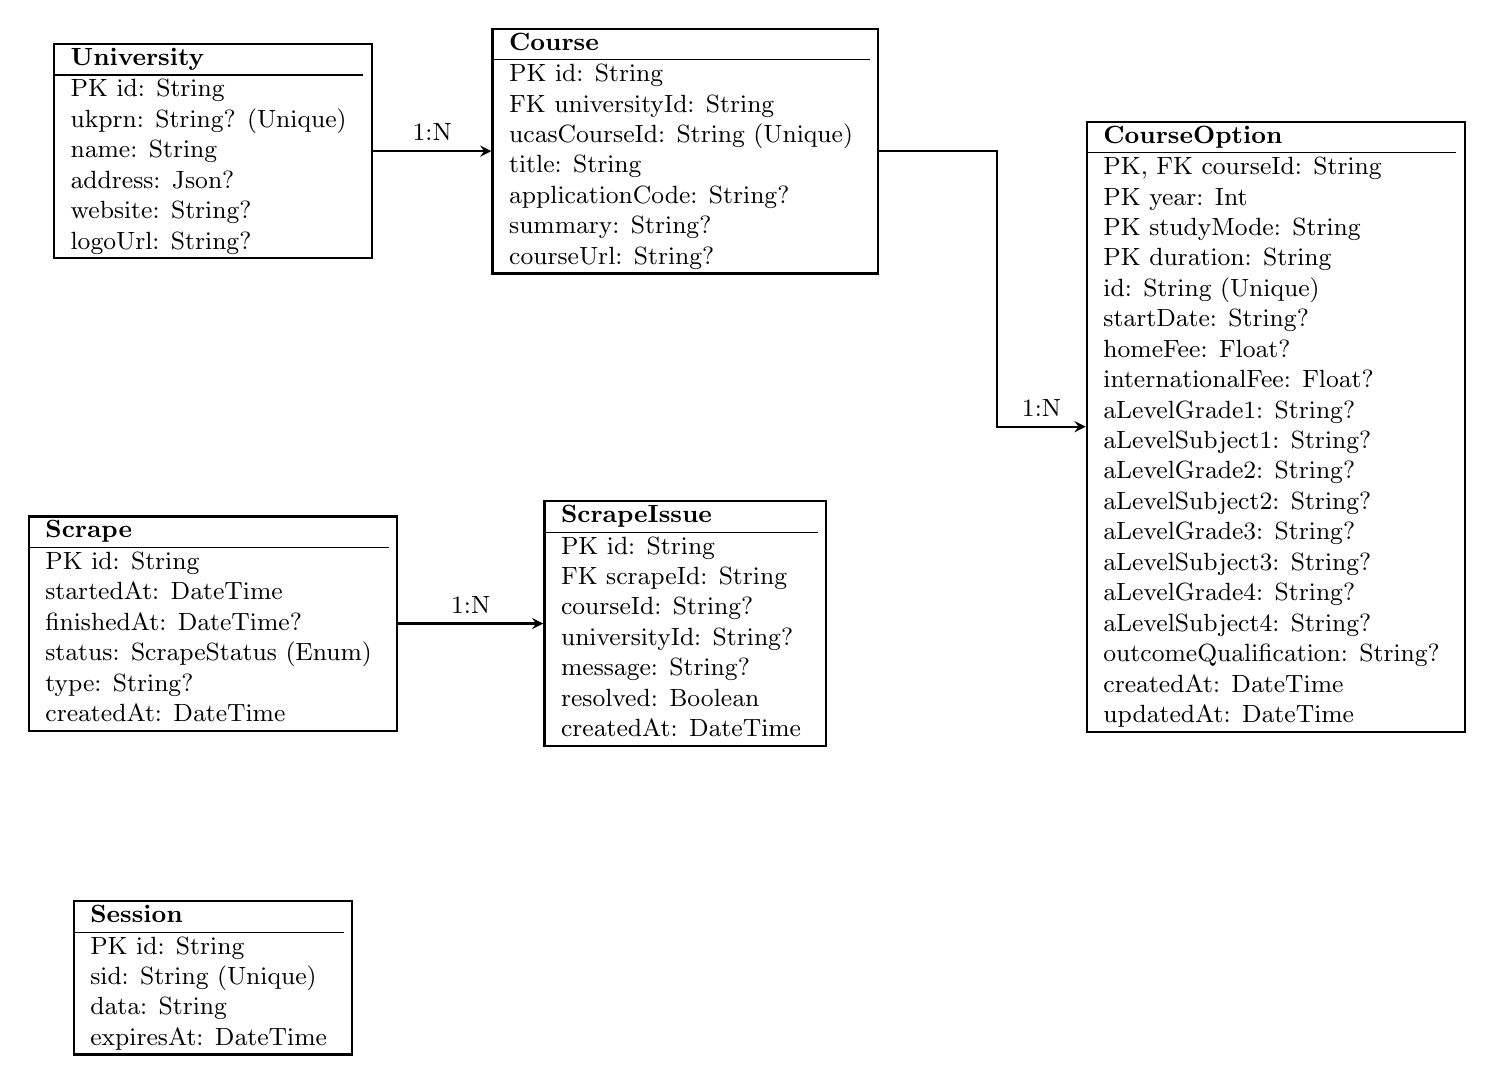
\begin{tikzpicture}[>=stealth, font=\small]
        
        % -----------------------
        % 1. University Node
        % -----------------------
        \node[draw, thick, inner sep=0pt, align=left] (uni) at (0, 0) {
            \begin{tabular}{l}
                \textbf{University} \\
                \hline
                PK id: String \\
                ukprn: String? (Unique) \\
                name: String \\
                address: Json? \\
                website: String? \\
                logoUrl: String? \\
            \end{tabular}
        };

        % -----------------------
        % 2. Course Node
        % -----------------------
        \node[draw, thick, inner sep=0pt, align=left] (course) at (6, 0) {
            \begin{tabular}{l}
                \textbf{Course} \\
                \hline
                PK id: String \\
                FK universityId: String \\
                ucasCourseId: String (Unique) \\
                title: String \\
                applicationCode: String? \\
                summary: String? \\
                courseUrl: String? \\
            \end{tabular}
        };

        % -----------------------
        % 3. CourseOption Node (Very Tall)
        % -----------------------
        \node[draw, thick, inner sep=0pt, align=left] (option) at (13.5, -3.5) {
            \begin{tabular}{l}
                \textbf{CourseOption} \\
                \hline
                PK, FK courseId: String \\
                PK year: Int \\
                PK studyMode: String \\
                PK duration: String \\
                id: String (Unique) \\
                startDate: String? \\
                homeFee: Float? \\
                internationalFee: Float? \\
                aLevelGrade1: String? \\
                aLevelSubject1: String? \\
                aLevelGrade2: String? \\
                aLevelSubject2: String? \\
                aLevelGrade3: String? \\
                aLevelSubject3: String? \\
                aLevelGrade4: String? \\
                aLevelSubject4: String? \\
                outcomeQualification: String? \\
                createdAt: DateTime \\
                updatedAt: DateTime \\
            \end{tabular}
        };

        % -----------------------
        % 4. Scrape Node
        % -----------------------
        \node[draw, thick, inner sep=0pt, align=left] (scrape) at (0, -6) {
            \begin{tabular}{l}
                \textbf{Scrape} \\
                \hline
                PK id: String \\
                startedAt: DateTime \\
                finishedAt: DateTime? \\
                status: ScrapeStatus (Enum) \\
                type: String? \\
                createdAt: DateTime \\
            \end{tabular}
        };

        % -----------------------
        % 5. ScrapeIssue Node
        % -----------------------
        \node[draw, thick, inner sep=0pt, align=left] (issue) at (6, -6) {
            \begin{tabular}{l}
                \textbf{ScrapeIssue} \\
                \hline
                PK id: String \\
                FK scrapeId: String \\
                courseId: String? \\
                universityId: String? \\
                message: String? \\
                resolved: Boolean \\
                createdAt: DateTime \\
            \end{tabular}
        };

        % -----------------------
        % 6. Session Node (Standalone)
        % -----------------------
        \node[draw, thick, inner sep=0pt, align=left] (session) at (0, -10.5) {
            \begin{tabular}{l}
                \textbf{Session} \\
                \hline
                PK id: String \\
                sid: String (Unique) \\
                data: String \\
                expiresAt: DateTime \\
            \end{tabular}
        };

        % -----------------------
        % Relationships (Lines)
        % -----------------------
        % University -> Course (Straight horizontal line)
        \draw[->, thick] (uni.east) -- node[above] {1:N} (course.west);
        
        % Course -> CourseOption (Orthogonal step line: goes right, then down, then right)
        \draw[->, thick] (course.east) -- ++(1.5,0) |- node[near end, above] {1:N} (option.west);
        
        % Scrape -> ScrapeIssue (Straight horizontal line)
        \draw[->, thick] (scrape.east) -- node[above] {1:N} (issue.west);

    \end{tikzpicture}
    } % End of resizebox
    \caption{Entity Relationship Diagram (ERD) mapping the complete Prisma database schema.}
    \label{fig:erd}
\end{figure}

\subsubsection{Scraping Engine Architecture}
The core technical challenge was managing the diversity of 35 different university websites. To solve this, we implemented the \textbf{Adapter Pattern} within the Scraping Engine.

The \texttt{Manager} class acts as the client. It iterates through the configuration list and instantiates a scraper based on the university's requirements.
\begin{enumerate}
    \item \textbf{GenericHtmlAdapter:} The default adapter. It uses \texttt{Cheerio} for fast static parsing and falls back to \texttt{Puppeteer} if dynamic content is detected.
    \item \textbf{Specific Adapters (e.g., EdinburghAdapter):} These extend the generic adapter to handle edge cases, such as the University of Edinburgh's Single Page Application (SPA) structure, where fee data is hidden behind dynamic redirects.
\end{enumerate}

This polymorphic design ensures that adding a new university only requires writing a new Adapter class, without modifying the core Engine logic.

% --- FIGURE: CLASS DIAGRAM (TIKZ) ---
\begin{figure}[h!]
    \centering
    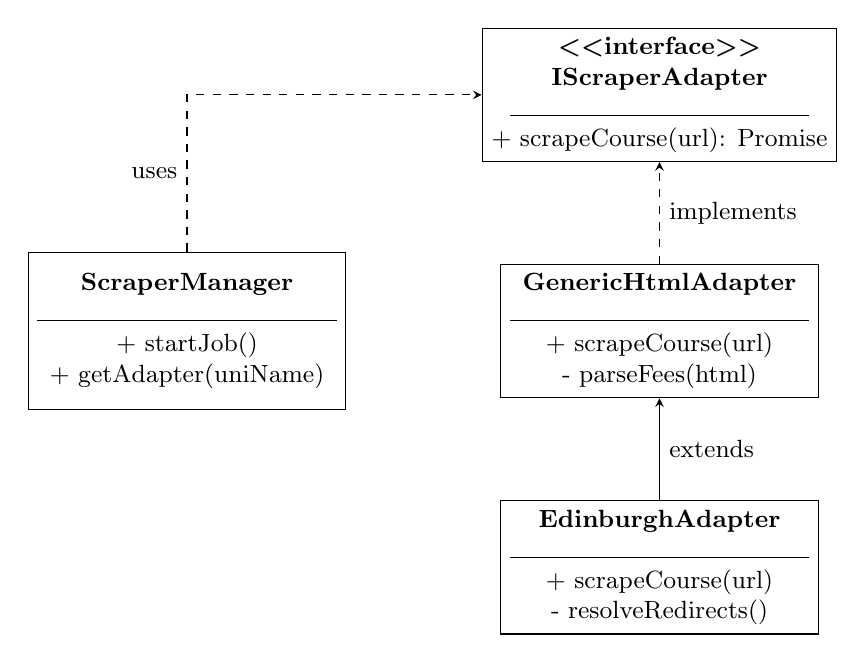
\begin{tikzpicture}[>=stealth, font=\small]
        % Interface
        \node[draw, rectangle, minimum width=4cm, minimum height=1.5cm, align=center] (interface) at (0, 0) {
            \textbf{\textless\textless interface\textgreater\textgreater} \\
            \textbf{IScraperAdapter} \\
            \rule{3.8cm}{0.4pt} \\
            + scrapeCourse(url): Promise
        };

        % Generic Adapter
        \node[draw, rectangle, minimum width=4cm, minimum height=1.5cm, align=center] (generic) at (0, -3) {
            \textbf{GenericHtmlAdapter} \\
            \rule{3.8cm}{0.4pt} \\
            + scrapeCourse(url) \\
            - parseFees(html)
        };

        % Specific Adapter
        \node[draw, rectangle, minimum width=4cm, minimum height=1.5cm, align=center] (specific) at (0, -6) {
            \textbf{EdinburghAdapter} \\
            \rule{3.8cm}{0.4pt} \\
            + scrapeCourse(url) \\
            - resolveRedirects()
        };

        % Scraper Manager
        \node[draw, rectangle, minimum width=4cm, minimum height=2cm, align=center] (manager) at (-6, -3) {
            \textbf{ScraperManager} \\
            \rule{3.8cm}{0.4pt} \\
            + startJob() \\
            + getAdapter(uniName)
        };

        % Relations
        \draw[->, dashed] (generic) -- node[midway, right] {implements} (interface);
        \draw[->] (specific) -- node[midway, right] {extends} (generic);
        % L-shaped arrow from manager to interface
        \draw[->, dashed] (manager.north) |- node[near start, left] {uses} (interface.west); 
    \end{tikzpicture}
    \caption{Class Diagram of the Scraper Engine demonstrating the Adapter Pattern.}
    \label{fig:class_diagram}
\end{figure}

\subsubsection{Technologies and Platforms}
We selected a unified \textbf{TypeScript} stack for both backend and frontend. This decision directly addresses the feedback regarding a "coherent technical stack":

\begin{itemize}
    \item \textbf{Type Safety:} Sharing TypeScript interfaces (DTOs) between the Backend and Frontend ensures that if the database schema changes, the frontend build will fail immediately, preventing runtime errors in production.
    \item \textbf{Backend (Node.js/Express):} Chosen over Python (originally considered) because it allows for non-blocking I/O, which is essential when scraping multiple websites concurrently.
    \item \textbf{Database (PostgreSQL \& Prisma):} PostgreSQL was chosen for its strict schema enforcement compared to NoSQL alternatives. Prisma acts as the bridge, generating type-safe database clients automatically.
\end{itemize}

\subsubsection{Role of Behaviour-Driven Development (BDD)}
The BDD approach bridged the gap between SPIO's requirements and our implementation. The Gherkin features defined in the Requirements Documentation served as the specification for our API Controllers.

For example, the requirement \textit{"Given I am a logged-in user... When I click Fetch Data..."} directly mapped to the \texttt{ScraperController}. We ensured that the code explicitly handled the authentication check (`Given`) before initiating the job queue (`Then`).

\begin{lstlisting}[language=Gherkin, caption={BDD-Driven Controller Logic}, label={lst:bdd_controller}]
// src/controllers/ScraperController.ts
// Maps to Feature: Fetching Data
router.post('/start', requireAuth, async (req, res) => {
    // "Given I am a logged-in user" -> handled by isAuthenticated middleware
    try {
        // "When I click Fetch Data" -> trigger the manager
        const jobId = await ScraperManager.startJob(req.body.universities);
        
        // "Then I should see a notification" -> return 200 OK
        res.status(200).json({ message: "Data fetch started", jobId });
    } catch (error) {
        res.status(500).json({ error: "Fetch failed" });
    }
});
\end{lstlisting}

\subsection{Usability and User Experience (5\%)}
As an internal enterprise tool replacing a manual workflow, our User Experience strategy prioritised \textbf{efficiency, data trust, and cognitive load reduction}. We addressed usability through the following key sub-features and design decisions:

\begin{enumerate}
    \item \textbf{System Visibility and Asynchronous Feedback:} Data scraping is a long-running process. To prevent users from assuming the system has frozen, leading to frustrated page refreshes, we implemented a robust feedback loop. HTTP-polling the \texttt{/api/scraper/status} endpoint provides real-time progress updates (e.g., \textit{"Scraping is running, 0 issues discovered..."}).
    
    \item \textbf{Error Resilience and Graceful Degradation:} If a specific university's scraper fails due to website layout changes or bot-protection, the system does not crash the entire batch. Instead, the backend logs the error to the \texttt{ScrapeIssue} table and continues processing. The UI highlights these specific failures post-scrape, allowing analysts to immediately export and use the successful data.
    
    \item \textbf{Advanced Course Lookup and Faceted Filtering:} To help analysts navigate thousands of courses without needing to export to Excel first, we implemented a highly responsive dynamic data grid featuring:
    \begin{itemize}
        \item \textbf{Debounced Searching:} Efficient database queries without lagging the UI, allowing instant keyword lookups (e.g., "Cyber Security").
        \item \textbf{Multi-criteria Filtering:} Stackable filters (fee ranges, study modes, competitor brackets) to narrow down 10,000+ courses to a target segment in seconds.
    \end{itemize}

    \item \textbf{Contextual Drill-Down:} Clicking any course row opens a comprehensive "Detailed View". This isolates the course to present historical fee comparisons, granular entry requirements, and crucially, a direct hyperlink to the \textit{original source URL}. Providing this source link builds absolute trust, allowing analysts to manually verify the scraped data if an anomaly appears.
    
    \item \textbf{Familiarity and Reduced Learning Curve:} To ensure high user adoption, dashboards and data tables were explicitly styled to mimic SPIO's existing market intelligence tools. Familiar iconography, standard pagination, and an "Export to Excel" pipeline that matches their current workflows ensure staff can transition to this application with near-zero onboarding time.
\end{enumerate}